\documentclass[twocolumn]{aastex631}

\usepackage{amsmath,amssymb}
\usepackage{graphicx}
\usepackage{booktabs}
\usepackage{multirow}
\usepackage{tabularx}
\usepackage{hyperref}
\usepackage{natbib}

\shorttitle{Structure-Aware Deep Learning for Radio Image Reconstruction}
\shortauthors{Hu et al.}

\begin{document}

\title{Structure-Aware Multimodal Learning for Radio Interferometric Image Reconstruction}

\author{ZHIFA HU}
\affiliation{School of Mechatronic Engineering and Automation, Shanghai University, Shanghai, China}
\affiliation{Chengdu Eapil Technology Co., Ltd., Chengdu, China}

\author{ENZE ZHANG}
\affiliation{School of Mechatronic Engineering and Automation, Shanghai University, Shanghai, China}
\affiliation{Chengdu Eapil Technology Co., Ltd., Chengdu, China}

\author{FANYI MENG}
\affiliation{Department of Astronomy, Tsinghua University, Beijing, China}

\author{JIANYONG ZHENG}
\affiliation{School of Mechatronic Engineering and Automation, Shanghai University, Shanghai, China}

\begin{abstract}
	Radio interferometric imaging is an ill-posed inverse problem because incomplete $uv$ coverage produces dirty images in which sky emission is convolved with a sidelobe-rich point spread function (PSF).
	Although CLEAN and its variants remain the practical standard, their computational and tuning costs can become substantial for large survey-scale imaging.
	This work presents a structure-aware multimodal reconstruction framework that jointly uses dirty images, PSFs, and single-dish (SD) observations.
	The study emphasizes three design factors that are especially important for radio data: dynamic-range-aware normalization, explicit conditioning on the instrumental response, and structure-aware training losses.
	On 12,726 CASA-simulated VLA image samples, four normalization schemes, six network backbones, and multiple ablation settings are evaluated under a unified protocol.
	Independent per-source normalization yields the most stable optimization, and adding gradient- and Laplacian-based structure terms improves reconstruction more than architecture scaling alone.
	The best model, a larger U-Net with the composite loss, reaches 28.46\,dB PSNR and 0.836 SSIM on a shared 1,272-sample evaluation split, improving over the simple U-Net baseline by +2.31\,dB.
	For context, CASA \texttt{tclean} references without SD conditioning reach 11.54\,dB PSNR for H{\"o}gbom CLEAN and 11.55\,dB for multi-scale CLEAN under the same split and normalization protocol.
	Matched architecture-level ablations further show that removing SD input causes a 12.9--14.0\,dB PSNR drop, indicating that low-spatial-frequency information is a major contributor to the final image quality.
	These results support structure-aware multimodal learning as a practical high-fidelity complement to classical radio-imaging workflows.
	Code and reproducibility resources are available at \url{https://github.com/arctanbell/radio_recon.git}.
\end{abstract}

\keywords{methods: data analysis --- techniques: image processing --- techniques: interferometric --- radio continuum: general --- methods: numerical}

% ============================================================
\section{Introduction}
\label{sec:intro}

Radio interferometers measure spatial-frequency samples of the sky brightness by correlating signals from separated antenna pairs, enabling angular resolutions beyond those of single-dish telescopes.
Because the available baselines are finite and non-uniform, the $uv$ plane is sampled incompletely.
The resulting dirty image can be viewed as the true sky brightness convolved with the synthesized beam, or dirty beam, plus noise, so sidelobes and missing short-spacing information distort extended and faint emission \citep{Thompson2017}.

Recovering a high-fidelity estimate of the sky brightness from dirty images is therefore an ill-posed inverse problem.
The CLEAN family remains the practical standard, including multi-scale variants, but its performance depends on iterative deconvolution choices, masking, stopping criteria, and other imaging parameters \citep{Hogbom1974,Cornwell2008}.
Alternative regularized approaches, including compressed-sensing and Bayesian formulations, provide more explicit inverse-problem treatments, but many are computationally demanding for large imaging workloads \citep{Wiaux2009,Li2011,Carrillo2012,Junklewitz2016,Arras2019}.

Learning-based methods have increasingly been applied to radio-interferometric image reconstruction.
Existing studies include CNN-based radio-image enhancement, residual image restoration, plug-and-play learned regularization, and generative or unrolled inverse-problem formulations \citep{Gheller2018,Schmidt2022,Connor2022,Terris2022,Aghabiglou2024,Wang2023VICDDPM,Geyer2023}.
Despite this progress, it remains less clear which design choices matter most when supervised models are trained for survey-scale image-domain reconstruction.
Four issues are particularly relevant:
(1) radio images can span several orders of magnitude in dynamic range, making normalization a first-order training decision;
(2) observation-dependent PSFs encode information about the $uv$ coverage and should be available to the reconstruction model;
(3) SD maps provide short-spacing and low-spatial-frequency information, but their contribution is not often isolated in learned reconstruction benchmarks;
and (4) structure-preserving losses, model capacity, and modality ablations are seldom evaluated together under one protocol.

A structure-aware multimodal learning framework is developed and evaluated under a unified benchmark to address these challenges.
The main contributions are as follows:
\begin{enumerate}
	\item A supervised multimodal reconstruction formulation is evaluated that jointly conditions on dirty images, PSFs, and SD maps, allowing the network to use complementary instrumental and low-spatial-frequency information.
	\item Four normalization strategies are compared systematically, showing that independent per-source normalization is a key factor for stable optimization on extreme-dynamic-range radio data.
	\item A composite objective combining pixel-domain, Fourier-domain, and structure-aware differential terms is evaluated and shown to improve structural fidelity more effectively than increasing model capacity alone.
	\item A unified benchmark spanning six CNN/Transformer backbones and 12,726 simulated image samples is established, including CASA \texttt{tclean} references and matched ablations that isolate the effects of SD input and training-sample filtering.
	\item The resulting analysis separates the roles of normalization, loss design, model capacity, and auxiliary data, providing a benchmark reference for future radio-imaging learning systems.
\end{enumerate}

% ============================================================
\section{Related Work}
\label{sec:related}

\subsection{Classical Radio Image Reconstruction}

The CLEAN algorithm \citep{Hogbom1974} remains the most widely used family of deconvolution methods in radio astronomy.
Subsequent variants include Clark CLEAN \citep{Clark1980}, Cotton--Schwab CLEAN \citep{Schwab1984}, and multi-scale CLEAN \citep{Cornwell2008}, each improving a different aspect of the original component-subtraction procedure.
The W-projection algorithm \citep{Cornwell2008WProjection} addresses non-coplanar wide-field imaging effects, while multi-frequency synthesis \citep{Rau2011} exploits spectral information during imaging.
Maximum entropy methods (MEM) \citep{Cornwell1985} provide an alternative regularized reconstruction framework, although they can over-smooth compact or complex structure depending on the data and regularization.
Beyond deconvolution itself, modern radio-imaging pipelines are tightly coupled to calibration and wide-field solvers based on the radio interferometer measurement equation \citep{Smirnov2011}.
Practical systems such as WSClean and DDFacet are widely used in large surveys \citep{Offringa2014,Tasse2018}.
This broader context is important because the CASA \texttt{tclean} experiments in this paper are intended as reproducible classical references rather than an exhaustive comparison against all modern imaging pipelines.

\subsection{Deep Learning for Interferometric Imaging}

Learning-based approaches to radio image reconstruction can be grouped roughly into three lines of work.
\emph{Post-processing and image-domain methods} apply neural networks to enhance CLEAN outputs or map dirty images to sky-model-like targets, treating reconstruction as image-to-image restoration \citep{Gheller2018,Schmidt2022,Geyer2023,Zhou2025UNet}.
\emph{End-to-end and learned inverse-problem methods} learn reconstruction operators from dirty images, visibilities, or residual measurement-domain information \citep{Connor2022,Aghabiglou2024,Wang2023VICDDPM}.
\emph{Physics-informed learned-regularization methods} incorporate the measurement equation through unrolled optimization or plug-and-play denoisers, including the AIRI family \citep{Terris2022,Terris2025AIRI}.
Recent progress in generative reconstruction is also related to diffusion modeling \citep{Ho2020DDPM,Song2021ScoreSDE}, and to inverse-problem priors such as plug-and-play and RED regularization \citep{Venkatakrishnan2013,Romano2017}.

This literature shows that learning-based radio-interferometric imaging is already an active research area.
The present work therefore does not claim to introduce deep learning to radio imaging for the first time.
Instead, it focuses on a deterministic, SD-conditioned supervised formulation in which dirty images, PSFs, and SD maps are provided jointly, and it quantifies normalization, loss, SD-input, and CASA \texttt{tclean} effects under one shared benchmark.

The VIC-DDPM method \citep{Wang2023VICDDPM} is particularly relevant to this setting.
It conditions diffusion sampling on both visibility-domain measurements and dirty images, and reports stronger recovery of faint sources and fine structures than several classical and deep-learning baselines.
Compared with VIC-DDPM, the present method focuses on deterministic one-pass reconstruction with explicit structure-aware differential loss terms and multimodal image-domain conditioning (PSF, dirty image, and SD map), targeting efficient large-scale batch inference rather than iterative generative sampling.

U-Net architectures \citep{Ronneberger2015} have been widely adopted for image restoration tasks.
Vision Transformers, including SwinIR \citep{Liang2021}, have shown strong performance on natural-image super-resolution and denoising and provide useful high-capacity baselines for reconstruction experiments.
Diffusion Transformers (DiT) \citep{Peebles2023} further motivate transformer-based generative modeling, although the present experiments use deterministic reconstruction rather than diffusion sampling.
From a broader inverse-problem viewpoint, compressed sensing theory \citep{Candes2006,Donoho2006} motivates sparse and structure-preserving priors, complementing the differential losses evaluated in this work.

\subsection{Multimodal Conditioning}

Feature-wise Linear Modulation (FiLM) \citep{Perez2018} provides a lightweight mechanism for conditioning neural networks on auxiliary inputs by predicting channel-wise scale and shift parameters.
Cross-attention mechanisms \citep{Vaswani2017} offer a more flexible alternative that can adapt features spatially to a conditioning signal.
In radio astronomy, combining interferometric and single-dish data is a long-standing strategy for recovering both high angular resolution and short-spacing information \citep{Plunkett2023}.
Traditional combinations are usually implemented through feathering, joint deconvolution, or visibility/image-domain data-combination workflows.
In this work, the SD map is instead used as an explicit conditioning channel in a supervised neural reconstruction model.
This use of SD information is therefore best interpreted as a learned image-domain conditioning strategy, not as a replacement for calibration, feathering, or joint deconvolution in a complete radio-imaging pipeline.

% ============================================================
\section{Method}
\label{sec:method}

\subsection{Problem Formulation}

Given a dirty image $D$, its corresponding dirty beam or PSF $B_{\mathrm{D}}$, and an associated single-dish map $I_{\mathrm{SD}}$, the learning objective is to predict a benchmark reference target $I_{\mathrm{ref}}^*$.
The interferometric dirty image can be described, under a calibrated small-field image-domain approximation, as
\begin{equation}
	D(\mathbf{x}) = \left(I_{\mathrm{sky}} \ast B_{\mathrm{D}}\right)(\mathbf{x}) + \epsilon(\mathbf{x}),
	\label{eq:measurement}
\end{equation}
where $I_{\mathrm{sky}}$ is the latent sky brightness, $B_{\mathrm{D}}$ is the dirty beam induced by the sampled and weighted $uv$ coverage, $\ast$ denotes convolution, and $\epsilon$ denotes effective noise and residual imaging errors.
Equivalently, in the Fourier domain,
\begin{equation}
	\tilde{D}(\mathbf{u}) = \tilde{B}_{\mathrm{D}}(\mathbf{u})\,\tilde{I}_{\mathrm{sky}}(\mathbf{u}) + \tilde{\epsilon}(\mathbf{u}),
	\label{eq:measurement_fourier}
\end{equation}
where $\tilde{B}_{\mathrm{D}}$ represents the sampling and weighting response.
The supervised reconstruction model is then defined as
\begin{equation}
	\hat{I}_{\mathrm{ref}} = f_\theta(D, B_{\mathrm{D}}, I_{\mathrm{SD}}),
\end{equation}
and is trained to minimize a composite loss between $\hat{I}_{\mathrm{ref}}$ and $I_{\mathrm{ref}}^*$.
Here, $I_{\mathrm{ref}}^*$ is the benchmark reference product produced by the simulation and imaging pipeline, not a directly observed true sky image.

The three input modalities are concatenated channel-wise to form a 3-channel input tensor $\mathbf{X} \in \mathbb{R}^{3 \times H \times W}$, where the channels correspond to $B_{\mathrm{D}}$, $D$, and $I_{\mathrm{SD}}$, respectively.
The output is a single-channel prediction $\hat{I}_{\mathrm{ref}} \in \mathbb{R}^{1 \times H \times W}$.

\subsection{Normalization Strategies}
\label{sec:normalization}

Radio astronomical images exhibit extreme dynamic ranges: the raw dirty-image and reference-target amplitudes can differ by more than $10^4$ within a sample, and the reference-target dynamic range varies strongly across the dataset.
Normalization is therefore a first-order training decision rather than a cosmetic preprocessing step.

Four strategies are investigated.
For compact notation, define the percentile min--max operator
\begin{equation}
	\mathcal{N}(x) =
	\mathrm{clip}\left(\frac{x - p_1(x)}{p_{99}(x) - p_1(x)}, 0, 1\right),
\end{equation}
where $p_1(x)$ and $p_{99}(x)$ denote the 1st and 99th percentiles of the finite pixels of $x$.

\paragraph{Independent Normalization (Recommended).}
Each sample and modality is normalized separately in normalized image space:
\begin{equation}
	\hat{D}=\mathcal{N}(D), \quad
	\hat{I}_{\mathrm{SD}}=\mathcal{N}(I_{\mathrm{SD}}), \quad
	\hat{I}_{\mathrm{ref}}^*=\mathcal{N}(I_{\mathrm{ref}}^*).
\end{equation}
The PSF is first normalized by its total sum and then percentile-scaled,
\begin{equation}
	\hat{B}_{\mathrm{D}}=\mathcal{N}\left(B_{\mathrm{D}} / \sum_{\mathbf{x}} B_{\mathrm{D}}(\mathbf{x})\right).
\end{equation}
This strategy maximizes the usable contrast of the reference target in the normalized training space while keeping the input channels numerically comparable.

\paragraph{Ratio-Preserving Normalization.}
The dirty image and reference target share a common percentile range estimated from their pooled pixels.
This preserves their relative amplitude scale, but can compress the reference target when the dirty image has a much larger amplitude range.

\paragraph{Arcsinh Normalization.}
A nonlinear $\mathrm{arcsinh}(x/\sigma)$ transform is applied before percentile scaling, where $\sigma$ is the per-sample standard deviation.
This is motivated by the common use of arcsinh scaling for visualizing high-dynamic-range astronomical images.

\paragraph{Adaptive Normalization.}
A hybrid strategy applies arcsinh scaling to the dirty image, median absolute deviation (MAD) robust scaling to the SD image, and independent percentile scaling to the reference target.

\subsection{Model Architectures}
\label{sec:architectures}

Six representative architectures spanning CNN and Transformer families are evaluated.

\subsubsection{Simple U-Net (Baseline)}

The baseline is a supervised U-Net \citep{Ronneberger2015} that maps the concatenated input tensor $(B_{\mathrm{D}}, D, I_{\mathrm{SD}})$ to a single-channel reference-target prediction.
It uses convolutional encoder--decoder blocks with skip connections, batch normalization, ReLU activations, and bilinear upsampling.
The default baseline configuration uses feature dimensions $[64, 128, 256, 512]$.

\subsubsection{Larger U-Net}

To test the effect of model capacity, an enlarged U-Net variant increases the feature dimensions to $[128, 256, 512, 1024]$ while keeping the same supervised input--output formulation.
This model isolates whether higher CNN capacity alone is sufficient to improve reconstruction quality.

\subsubsection{PSF-Conditioned U-Net Variants}

Two PSF-conditioned U-Net variants are included to test whether treating the PSF as an explicit conditioning signal improves over direct channel concatenation.
The FiLM-conditioned variant summarizes PSF features into channel-wise modulation parameters, while the cross-attention variant uses PSF-derived features as conditioning information for spatially adaptive feature fusion.
These variants evaluate whether more structured use of the instrumental response improves reconstruction beyond simple concatenation.

\subsubsection{SwinIR Transformer}

A SwinIR-style Transformer \citep{Liang2021} is adapted for radio image reconstruction by replacing the image-restoration input with the three-channel radio tensor.
The model uses shallow convolutional feature extraction, residual Swin Transformer stages with window-based self-attention, and a convolutional reconstruction head.
The large configuration uses an embedding dimension of 128, four stages, window size 8, and approximately 11.8M parameters.

\subsubsection{DiT-Style Transformer}

A patch-based Transformer inspired by Diffusion Transformers \citep{Peebles2023} is also evaluated as a deterministic reconstruction baseline.
Rather than performing diffusion sampling, the model maps input patches directly to a reconstructed image, allowing the experiment to test whether high-capacity patch-token processing benefits this supervised reconstruction setting.

\subsection{Composite Loss Function}
\label{sec:loss}

A composite supervised loss is used to combine pixel-domain accuracy, frequency-domain consistency, and morphology-aware differential regularization.
For a prediction $\hat{I}_{\mathrm{ref}}$ and reference target $I_{\mathrm{ref}}^*$, the pixel losses are
\begin{equation}
	\mathcal{L}_{\mathrm{MSE}} = \frac{1}{N}\sum_i
	\left(\hat{I}_{\mathrm{ref},i} - I_{\mathrm{ref},i}^*\right)^2,
	\quad
	\mathcal{L}_{L_1} = \frac{1}{N}\sum_i
	\left|\hat{I}_{\mathrm{ref},i} - I_{\mathrm{ref},i}^*\right|.
\end{equation}

The frequency-domain term compares log-magnitude Fourier spectra:
\begin{equation}
	\mathcal{L}_{\mathrm{FFT}} =
	\frac{1}{N_u}\sum_{\mathbf{u}}
	\left|
	\log\left(|\mathcal{F}\hat{I}_{\mathrm{ref}}(\mathbf{u})|+\epsilon\right)
	-
	\log\left(|\mathcal{F}I_{\mathrm{ref}}^*(\mathbf{u})|+\epsilon\right)
	\right|,
\end{equation}
where $\mathcal{F}$ denotes the 2D discrete Fourier transform and $\epsilon$ is a small numerical constant.

The structure-aware terms compare first- and second-order image derivatives:
\begin{equation}
	\mathcal{L}_{\mathrm{grad}} =
	\left\| \nabla_x \hat{I}_{\mathrm{ref}} - \nabla_x I_{\mathrm{ref}}^* \right\|_1
	+
	\left\| \nabla_y \hat{I}_{\mathrm{ref}} - \nabla_y I_{\mathrm{ref}}^* \right\|_1,
\end{equation}
\begin{equation}
	\mathcal{L}_{\mathrm{Lap}} =
	\left\| \nabla^2 \hat{I}_{\mathrm{ref}} - \nabla^2 I_{\mathrm{ref}}^* \right\|_1.
\end{equation}

The total loss is
\begin{equation}
	\mathcal{L} =
	\lambda_{\mathrm{MSE}}\mathcal{L}_{\mathrm{MSE}}
	+\lambda_{L_1}\mathcal{L}_{L_1}
	+\lambda_{\mathrm{FFT}}\mathcal{L}_{\mathrm{FFT}}
	+\lambda_{\mathrm{grad}}\mathcal{L}_{\mathrm{grad}}
	+\lambda_{\mathrm{Lap}}\mathcal{L}_{\mathrm{Lap}}.
	\label{eq:total_loss}
\end{equation}

The weights are configuration-specific rather than universal defaults.
The Simple U-Net structure-loss ablation uses $(0.30,0.20,0.20,0.15,0.15)$ for MSE, $L_1$, FFT, gradient, and Laplacian terms.
The main larger U-Net setting uses a lighter structure-aware recipe, $(0.46,0.30,0.20,0.02,0.02)$, to preserve stable pixel-level optimization.
SwinIR filtering experiments use the stronger structure-aware setting as an architecture-specific sensitivity check.
Thus, the differential losses are interpreted as morphology-aware image-domain regularizers, not as a full differentiable enforcement of the interferometric measurement equation.

\subsection{Reference-Target Dynamic-Range Filtering}
\label{sec:filtering}

Per-sample error analysis shows that a subset of samples consistently falls below 20\,dB PSNR across models.
These failures are concentrated in cases with extremely small reference-target dynamic range, where percentile normalization can amplify small numerical variations and weaken the effective supervision signal.
To evaluate this failure mode, training samples are ranked by the dynamic range of $I_{\mathrm{ref}}^*$, and the bottom 1--2\% are optionally excluded during training.
Unless explicitly stated otherwise, evaluation remains on the full shared benchmark split, so filtering is treated as a training-time robustness intervention rather than a test-time score adjustment.

% ============================================================
\section{Experiments}
\label{sec:experiments}

\subsection{Dataset}

A large-scale simulated benchmark generated with CASA \citep{CASA2022} is used.
The benchmark contains 12,726 valid image samples from VLA D-configuration simulations at 1.42\,GHz with 2\,kHz channel width.
Each simulation uses 7,200\,s of integration time with 10\,s integration intervals.

For each sample, four image products are used:
\begin{itemize}
	\item \textbf{Dirty image} ($D$): the primary-beam-corrected dirty image, stored as \texttt{\_dirty.image.pbcor.fits} when available, with \texttt{\_dirty.image.fits} used as fallback.
	\item \textbf{Dirty beam / PSF} ($B_{\mathrm{D}}$): the PSF associated with the sampled and weighted $uv$ coverage, stored as \texttt{\_dirty.psf.fits}.
	\item \textbf{Single-dish map} ($I_{\mathrm{SD}}$): the regridded single-dish or total-power image, stored as \texttt{\_rg\_fast.fits}.
	\item \textbf{Reference target} ($I_{\mathrm{ref}}^*$): the regridded \texttt{\_rg\_dirty.fits} product used as the supervised reconstruction target.
\end{itemize}

All images have a spatial size of $192 \times 192$ pixels.
The benchmark uses a fixed seed-42 train/validation/test partition with a 0.8/0.1/0.1 split at the sample level.
Unless otherwise noted, the primary benchmark reports the held-out 1,272-sample test split, and filtered protocols report their own scoring sample counts explicitly.

\subsection{Training Details}

Models are trained with AdamW \citep{Loshchilov2019}, weight decay $10^{-5}$, cosine learning-rate annealing, and mixed-precision training where supported.
The exact learning rate, batch size, and epoch count are configuration-specific.
The Simple U-Net normalization baseline uses 100 epochs, batch size 16, and an initial learning rate of $10^{-4}$.
The main larger U-Net setting uses 260 epochs, batch size 8, and an initial learning rate of $5\times10^{-5}$.
SwinIR large configurations use 400 epochs, batch size 4, and an initial learning rate of $10^{-4}$.

Data augmentation consists of random horizontal and vertical flips, random $90^\circ$ rotations, and additive Gaussian noise on the dirty-image channel when enabled by the experiment configuration.
The best checkpoint is selected using validation loss, and final metrics are reported on the held-out test split.
Multi-GPU jobs use PyTorch Distributed Data Parallel when applicable; single-GPU and multi-GPU runs follow the same dataset split and evaluation protocol.

\subsection{Evaluation Metrics}

The following metrics are reported between $\hat{I}_{\mathrm{ref}}$ and $I_{\mathrm{ref}}^*$ in the normalized reference-target space:
\begin{itemize}
	\item \textbf{PSNR} (Peak Signal-to-Noise Ratio, dB): computed with data range 1.0.
	\item \textbf{SSIM} (Structural Similarity Index): computed on normalized images to quantify structural similarity.
	\item \textbf{MSE} (Mean Squared Error): pixel-domain squared error in normalized space.
	\item \textbf{MAE} (Mean Absolute Error): pixel-domain absolute error in normalized space.
\end{itemize}

All metrics are computed per sample and then averaged across the test set.
Standard deviations are reported where full per-sample distributions are available.

\subsection{CASA \texttt{tclean} Baselines}

To compare the learned reconstructions with classical radio-imaging practice, two CASA \texttt{tclean} references are evaluated on the same 1,272-sample held-out test split.
For each test sample, the archived measurement set is re-imaged with CASA \texttt{tclean} using the same imaging geometry as the simulated dirty-image generation: \texttt{imsize=[192,192]}, \texttt{cell=5arcsec}, Briggs weighting with \texttt{robust=0.5}, \texttt{gridder=standard}, \texttt{specmode=mfs}, and primary-beam correction enabled.
Two deconvolution settings are used: H{\"o}gbom CLEAN with \texttt{niter=1000}, \texttt{gain=0.1}, and \texttt{threshold=1mJy}; and multi-scale CLEAN with the same stopping parameters and scales \texttt{[0,2,5]}.
The resulting primary-beam-corrected images are compared with $I_{\mathrm{ref}}^*$ using the same per-sample normalization and metric definitions as the neural baselines.
This should be read as a reproducible classical-imaging reference: no exhaustive CLEAN parameter sweep, feathering, or joint SD--interferometer imaging mode is attempted, and the \texttt{tclean} runs do not use the auxiliary SD map available to the learned multimodal models.

% ============================================================
\section{Results}
\label{sec:results}

\subsection{Normalization Strategy Comparison}

Table~\ref{tab:normalization} presents the results of the four normalization strategies, all using the same Simple U-Net baseline trained for 100 epochs.

\begin{table*}[t]
	\centering
	\caption{Comparison of normalization strategies using the Simple U-Net baseline.}
	\label{tab:normalization}
	\begin{tabular}{lccc}
		\toprule
		Strategy         & PSNR (dB)      & SSIM           & Val Loss       \\
		\midrule
		Independent      & \textbf{26.16} & 0.785          & \textbf{0.100} \\
		Adaptive         & 25.54          & 0.778          & 0.103          \\
		Arcsinh          & 24.22          & 0.742          & 0.101          \\
		Ratio-preserving & 22.61          & \textbf{0.880} & 0.193          \\
		\bottomrule
	\end{tabular}
\end{table*}

Independent normalization yields the highest PSNR (26.16\,dB) and the lowest validation loss (0.100), supporting the hypothesis that preserving reference-target contrast in normalized space is critical for supervised optimization.
The ratio-preserving strategy produces the highest SSIM (0.880) but the lowest PSNR (22.61\,dB), suggesting that the elevated SSIM mainly reflects smoother predictions rather than improved reference-target fidelity.
Figure~\ref{fig:norm_hist} shows the same trend in the underlying intensity distributions: independent per-sample, per-modality normalization retains substantially more weak-signal occupancy near the low-intensity tail than the global or joint alternatives.
Independent normalization is therefore adopted in all subsequent experiments.

	\begin{figure}[t]
		\centering
		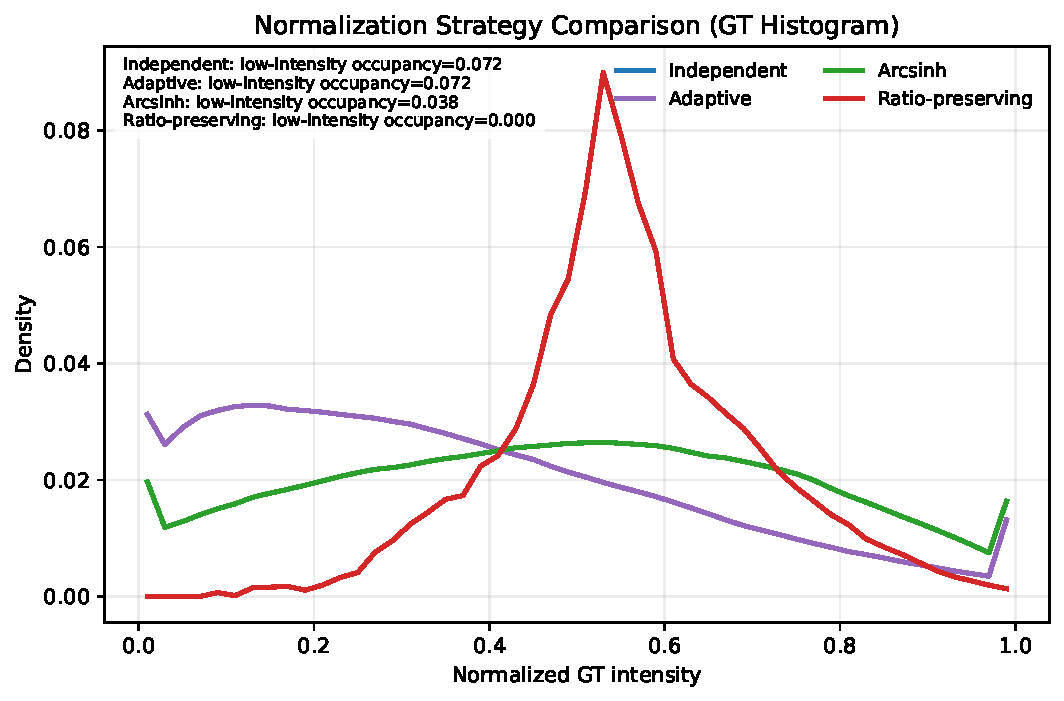
\includegraphics[width=\columnwidth]{figures/normalization_histogram_comparison.pdf}
		\caption{Dynamic-range histogram comparison of normalization strategies.
			Independent per-sample, per-modality normalization preserves weak-source occupancy and avoids excessive tail compression seen in global/joint normalization and pure log-style compression.
		}
		\label{fig:norm_hist}
	\end{figure}

\subsection{Architecture Comparison}

Table~\ref{tab:architecture} presents the comprehensive architecture comparison on the primary shared evaluation split (1,272 samples).

\begin{table*}[t]
	\centering
	\caption{Architecture comparison on the primary shared evaluation split (1,272 samples). All models use independent normalization and the composite loss function unless otherwise noted. $\Delta$PSNR is relative to the Simple U-Net baseline.}
	\label{tab:architecture}
	\begin{tabular}{lccccc}
		\toprule
		Model                             & Loss              & PSNR (dB)                 & SSIM                       & $\Delta$PSNR (dB) & Params             \\
		\midrule
		Simple U-Net [64--512]            & MSE+L1+FFT        & 26.16 $\pm$ 4.01          & 0.785 $\pm$ 0.156          & ---               & $\sim$7.8M         \\
		Simple U-Net [64--512]            & +Struct.          & 27.40                     & 0.810                      & +1.24             & $\sim$7.8M         \\
		Larger U-Net [128--1024]          & MSE+L1+FFT        & 26.62                     & 0.800                      & +0.46             & $\sim$31M          \\
		\textbf{Larger U-Net [128--1024]} & \textbf{+Struct.} & \textbf{28.46 $\pm$ 4.38} & \textbf{0.836 $\pm$ 0.141} & \textbf{+2.31}    & $\sim$\textbf{31M} \\
		FiLM U-Net [64--512]              & +Struct.          & 26.77                     & 0.800                      & +0.61             & $\sim$9.5M         \\
		SwinIR (small)                    & +Struct.          & 23.41                     & 0.760                      & $-$2.75           & $\sim$3.2M         \\
		SwinIR (large)                    & +Struct.          & 27.22                     & 0.820                      & +1.06             & $\sim$11.8M        \\
		DiT (large, patch=4)              & +Struct.          & 25.07 $\pm$ 3.77          & 0.761 $\pm$ 0.163          & $-$1.09           & $\sim$15M          \\
		\midrule
		\multicolumn{6}{l}{\textit{With reference-target filtering (train-only, 1\% threshold):}}                                                                                    \\
		SwinIR (large)                    & +Struct.          & 28.33 $\pm$ 4.83          & 0.832 $\pm$ 0.151          & +2.17             & $\sim$11.8M        \\
		\midrule
		\multicolumn{6}{l}{\textit{With reference-target filtering (train/val/evaluation, 1\% threshold, 1,259 evaluation samples):}}                                                \\
		SwinIR (large)                    & +Struct.          & 28.63 $\pm$ 5.17          & 0.833 $\pm$ 0.165          & +2.47             & $\sim$11.8M        \\
		\bottomrule
	\end{tabular}
\end{table*}


\paragraph{Structure-aware losses provide the largest isolated gain.}
Relative to the Simple U-Net baseline, adding gradient-matching and Laplacian terms improves PSNR by +1.24\,dB.
This indicates that morphology-aware supervision is a useful complement to pixel- and frequency-domain losses.

\paragraph{Model capacity helps, but is not sufficient alone.}
Increasing the U-Net width from $[64, 128, 256, 512]$ to $[128, 256, 512, 1024]$ provides +0.46\,dB.
Combining the larger U-Net with structure-aware losses gives the best result, reaching +2.31\,dB over the baseline.

\paragraph{Explicit PSF conditioning does not outperform simple concatenation in this benchmark.}
The FiLM-conditioned U-Net improves over the baseline by +0.61\,dB, but remains below the directly concatenated U-Net with structure-aware losses.
This suggests that preserving the PSF as a spatial input channel is more effective here than compressing it into global modulation features.

\paragraph{Transformer models are sensitive to capacity and protocol.}
The small SwinIR model underperforms substantially at 23.41\,dB, whereas the large SwinIR reaches 27.22\,dB.
With train-only reference-target filtering and extended training, the large SwinIR reaches 28.33\,dB on the same 1,272-sample shared evaluation split.
Under the separate filtered-evaluation protocol, it reaches 28.63\,dB on 1,259 samples.

\paragraph{Patch-based DiT is less effective for this setting.}
The DiT-style model reaches 25.07\,dB despite having about 15M parameters.
This suggests that the tested patch-token formulation is less well matched to local deconvolution-like structure recovery than skip-connected encoder--decoder models.

\subsection{Ablation Studies}

\subsubsection{Loss Function Components}

Table~\ref{tab:loss_ablation} presents a cumulative ablation of the loss components.

\begin{table}[htbp]
	\centering
	\caption{Cumulative loss-function ablation on the larger U-Net [128--1024].}
	\label{tab:loss_ablation}
	\begin{tabular}{lcc}
		\toprule
		Loss Configuration                    & PSNR (dB)     & $\Delta$      \\
		\midrule
		MSE only                              & 25.8          & ---           \\
		MSE + L1                              & 26.2          & +0.4          \\
		MSE + L1 + FFT                        & 26.6          & +0.8          \\
		MSE + L1 + FFT + Gradient + Laplacian & \textbf{28.5} & \textbf{+2.7} \\
		\bottomrule
	\end{tabular}
\end{table}

The structure-aware terms provide the largest incremental gain, adding about +1.9\,dB beyond the pixel- and frequency-domain losses.
This supports their usefulness for preserving structural detail in the normalized reference-target space.

\subsubsection{Reference-Target Dynamic-Range Filtering}

Table~\ref{tab:filtering} separates two uses of dynamic-range filtering: sensitivity checks that remove low-range samples from scoring, and stratified evaluation under a filtered SwinIR protocol.

\begin{table}[htbp]
	\centering
			\caption{Reference-target dynamic-range filtering and evaluation-set sensitivity analysis.
					Rows report the sample count used for scoring; protocols that remove samples from the evaluation set are not directly comparable to the fixed 1,272-sample benchmark.
				}
	\label{tab:filtering}
	\begin{tabular}{lccc}
		\toprule
			Condition           & Samples & PSNR (dB) & SSIM                                       \\
			\midrule
			\multicolumn{4}{l}{\textit{Larger U-Net, thresholded scoring set}} \\
			Full scoring set    & 1,272   & 28.46     & 0.836                                      \\
			Exclude bottom 0.5\%& 1,266   & 28.34     & 0.830                                      \\
			Exclude bottom 1\%  & 1,259   & 28.28     & 0.830                                      \\
			Exclude bottom 2\%  & 1,247   & 28.47     & 0.837                                      \\
			\midrule
			\multicolumn{4}{l}{\textit{Filtered SwinIR protocol, stratified scoring set}}                          \\
			Protocol scoring set& 1,259   & 28.63     & 0.833                                      \\
			Exclude bottom 1\%  & 1,234   & 28.74     & 0.840                                      \\
			Exclude bottom 5\%  & 1,184   & 29.10     & 0.850                                      \\
			Exclude bottom 10\% & 1,122   & 29.46     & 0.860                                      \\
		\bottomrule
	\end{tabular}
\end{table}

Removing low-dynamic-range samples from scoring changes the reported mean only modestly for the larger U-Net, with the 2\% filtered scoring set reaching 28.47\,dB on 1,247 samples compared with 28.46\,dB on the full 1,272-sample reference split.
The lower block shows the same phenomenon under the filtered SwinIR protocol: progressively removing the lowest-range samples increases the mean PSNR and SSIM, indicating that low-reference-range cases contribute disproportionately to the difficult tail of the benchmark.

\subsubsection{Test-Set Stratification by Dynamic Range}

To characterize model behavior across data-quality levels more directly, the scoring set is stratified by reference-target dynamic-range percentile (Table~\ref{tab:filtering}, lower block).

These results indicate that the lowest-dynamic-range samples disproportionately degrade the mean metrics.
On the top 90\% of the test set, the model reached 29.46\,dB PSNR and 0.860 SSIM, approaching the regime of high-quality image restoration.

\clearpage
\subsection{SD-Related Experimental Evidence}

To assess the practical value of SD-informed reconstruction, a unified benchmark is first constructed on the same 1,272-sample shared evaluation split.
Table~\ref{tab:sd_effect_proxy} and Figure~\ref{fig:sd_ablation_comp} compare CASA \texttt{tclean} references and dirty-only generic restorers against radio-tailored multimodal models that ingest PSF, dirty-image, and SD information.
Because this comparison changes architecture and training objective together with the input channels, it should be interpreted as a system-level benchmark rather than a strict causal ablation.
The comparison separates classical CLEAN, input-only references, dirty-only learned restoration, and SD-inclusive radio models, and it motivates the dedicated architecture-matched SD study below.

\begin{table*}[htbp]
	\centering
	\caption{Classical and learning-based references on a shared 1,272-sample evaluation split.
		CASA \texttt{tclean}, input-only images, and dirty-only methods are compared against multimodal radio models that include SD input.
	}
	\label{tab:sd_effect_proxy}
	\begin{tabular}{llcccc}
		\toprule
		Group     & Method             & PSNR (dB) & SSIM   & MSE      & MAE      \\
		\midrule
		\multicolumn{6}{l}{\textit{Classical radio reconstruction}}               \\
		Classical & CASA tclean (H{\"o}gbom)      & 11.54     & 0.2926 & 0.088575 & 0.233002 \\
		Classical & CASA tclean (multi-scale)     & 11.55     & 0.2942 & 0.088570 & 0.232990 \\
		\midrule
		\multicolumn{6}{l}{\textit{Input-only references}}                         \\
		Input     & Dirty image input              & 11.23     & 0.2748 & 0.093261 & 0.239891 \\
		Input     & SD image input                 & 19.04     & 0.6623 & 0.015924 & 0.087287 \\
		\midrule
		\multicolumn{6}{l}{\textit{Generic restoration (dirty-only input)}}       \\
		Generic   & DnCNN-standard     & 14.18     & 0.4516 & 0.045640 & 0.169785 \\
		Generic   & UNet-standard      & 14.60     & 0.4775 & 0.042880 & 0.162625 \\
		Generic   & SwinIR-standard    & 14.37     & 0.4676 & 0.044977 & 0.166429 \\
		\midrule
		\multicolumn{6}{l}{\textit{Radio deep learning (PSF+dirty+SD)}}           \\
		Radio DL  & FiLM U-Net    & 27.48     & 0.8127 & 0.002990 & 0.036380 \\
		Radio DL  & Structure-aware U-Net & 28.51     & 0.8364 & 0.002531 & 0.033158 \\
		Radio DL  & SwinIR       & 28.34     & 0.8324 & 0.002899 & 0.034910 \\
		\bottomrule
	\end{tabular}
\end{table*}

	\begin{figure}[htbp]
		\centering
		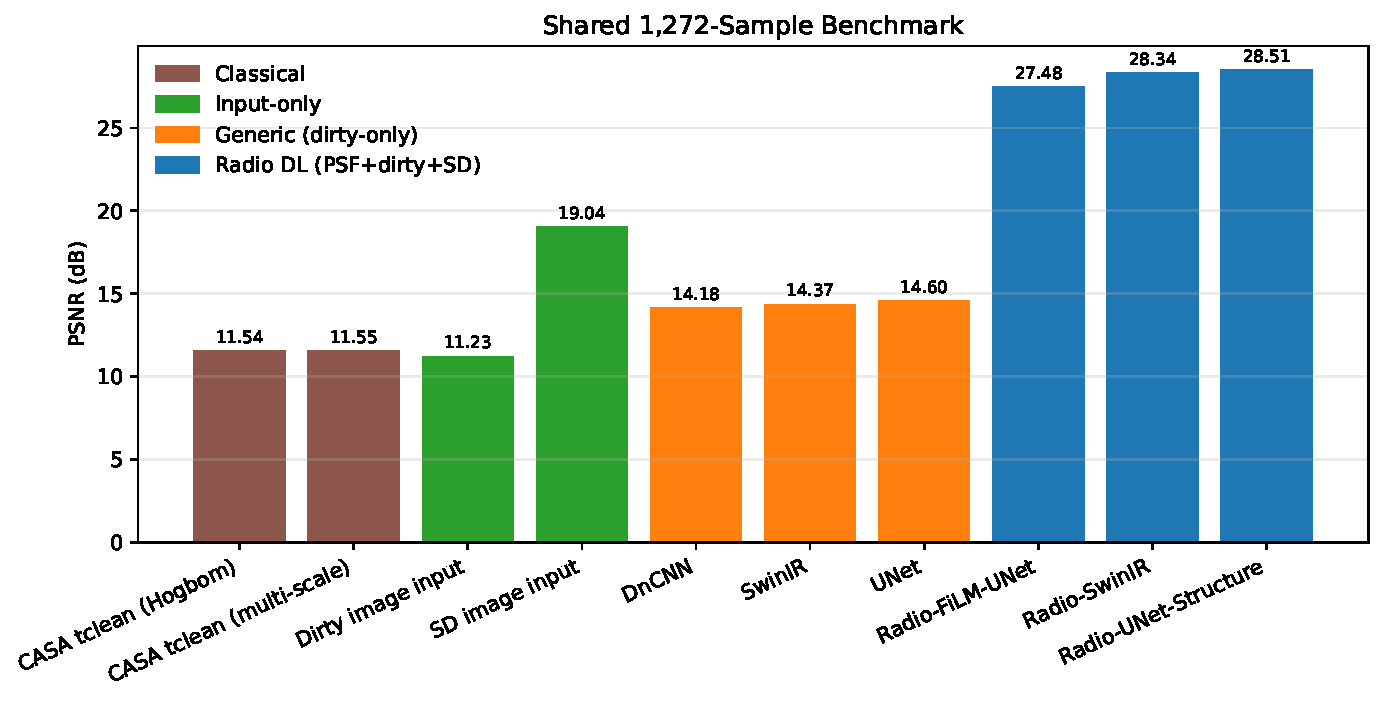
\includegraphics[width=\columnwidth]{figures/sd_ablation_comparison.pdf}
		\caption{Shared 1,272-sample benchmark comparison.
			The SD image input is already a strong reference, but multimodal radio models (PSF+dirty+SD) still outperform input-only, generic dirty-only, and CASA \texttt{tclean} references by large margins.
		}
		\label{fig:sd_ablation_comp}
	\end{figure}

The benchmark shows that radio-specific multimodal systems achieve markedly higher reference-target fidelity than both CASA \texttt{tclean} and dirty-only generic baselines across all four metrics.
The CASA H{\"o}gbom and multi-scale \texttt{tclean} references reach 11.54 and 11.55\,dB PSNR, respectively.
The direct SD image input reaches 19.04\,dB PSNR and 0.662 SSIM, indicating that SD carries substantial target-relevant large-scale information.
The strongest dirty-only generic models remain at 14.2--14.6\,dB PSNR, whereas the multimodal radio models occupy the 27.5--28.5\,dB regime.
The best model improves by 9.47\,dB over the SD-only input reference, indicating that the learned system is not simply copying the SD channel.
Because the benchmark varied input modality, model design, and training objective simultaneously, the specific contribution of SD was isolated separately through the architecture-matched ablation below.

\subsection{Architecture-Matched SD Training Ablation}

A controlled architecture-matched SD ablation is further performed by training each radio architecture in two modes: \textit{with SD} (PSF+dirty+SD) and \textit{PSF+dirty only}.
Results are reported in Table~\ref{tab:sd_train_ablation} and Figure~\ref{fig:sd_train_delta} on the same 1,272-sample shared evaluation split.

\begin{table*}[htbp]
	\centering
	\caption{Architecture-matched SD training ablation on identical backbones (1,272 evaluation samples).
		Each pair compares the same architecture trained with and without SD input.
	}
	\label{tab:sd_train_ablation}
	\begin{tabular}{lcccccc}
		\toprule
		Backbone     & Setting            & PSNR (dB) & SSIM   & MSE      & MAE      & $\Delta$PSNR \\
		\midrule
		FiLM U-Net    & with SD            & 27.48     & 0.8127 & 0.002990 & 0.036380 & +12.89       \\
		FiLM U-Net    & PSF+dirty only & 14.59     & 0.4764 & 0.044211 & 0.164286 & ---          \\
		\midrule
		Structure-aware U-Net & with SD            & 28.51     & 0.8364 & 0.002531 & 0.033158 & +13.89       \\
		Structure-aware U-Net & PSF+dirty only & 14.62     & 0.4778 & 0.042845 & 0.162547 & ---          \\
		\midrule
		SwinIR       & with SD            & 28.34     & 0.8324 & 0.002899 & 0.034910 & +13.99       \\
		SwinIR       & PSF+dirty only & 14.34     & 0.4660 & 0.044904 & 0.167074 & ---          \\
		\bottomrule
	\end{tabular}
\end{table*}

\begin{figure}[htbp]
	\centering
	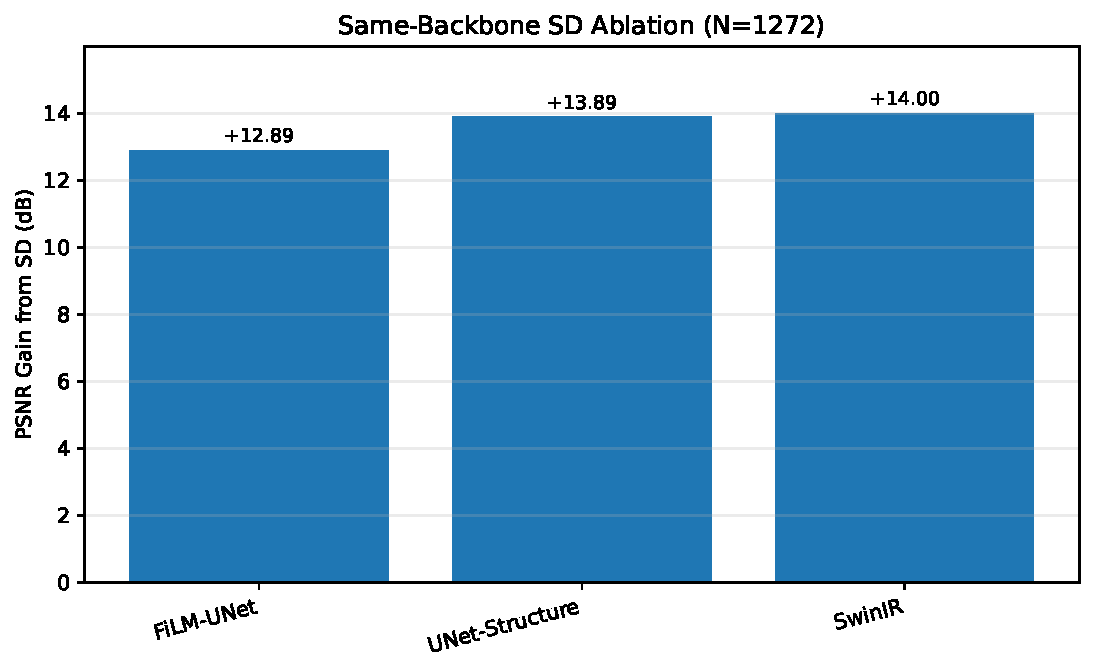
\includegraphics[width=\columnwidth]{figures/sd_training_delta_comparison.pdf}
	\caption{PSNR gain from SD input under architecture-matched training ablation.
		All three backbones show large improvements when SD is included.
	}
	\label{fig:sd_train_delta}
\end{figure}

The architecture-matched ablation indicates that SD input is a major contributor to reconstruction quality in this task.
Across all three backbones, removing SD during training reduces PSNR by 12.9--14.0\,dB and substantially worsens SSIM, while MSE and MAE increase by more than one order of magnitude.
The consistency of this effect across FiLM U-Net, structure-aware U-Net, and SwinIR suggests that the gain is not architecture-specific.
Instead, the SD channel supplies large-scale information that the interferometric inputs alone do not recover reliably under the present simulation setup.

\subsection{PSNR Distribution Analysis}

Figure~\ref{fig:psnr_distribution} illustrates the per-sample PSNR distribution for the best larger U-Net model.
The distribution is broad, spanning from approximately 16\,dB to over 35\,dB, with a standard deviation of $\pm$4.38\,dB.
Approximately 40\% of samples exceed 30\,dB, while $\sim$10\% fall below 20\,dB.
The low-PSNR tail correlates with reference-target dynamic range: samples with higher intrinsic dynamic range are reconstructed more accurately because normalization preserves a more usable learning signal.

\begin{figure}[htbp]
	\centering
	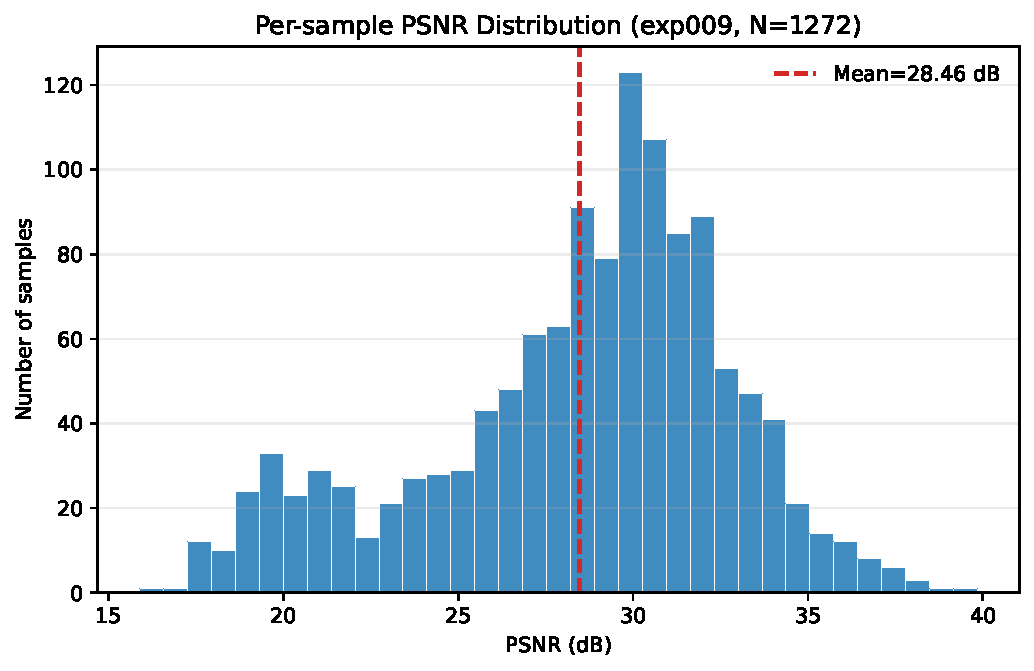
\includegraphics[width=\columnwidth]{figures/psnr_distribution.pdf}
		\caption{Per-sample PSNR distribution for the best larger U-Net model on 1,272 evaluation samples.
			The distribution spans $\sim$19\,dB, with $\sim$40\% of samples exceeding 30\,dB and $\sim$10\% below 20\,dB.
			Low-PSNR outliers correlate with low reference-target dynamic range.}
	\label{fig:psnr_distribution}
\end{figure}

\subsection{Qualitative Results}

Figure~\ref{fig:qualitative} presents representative reconstruction examples across different PSNR ranges.
For high-PSNR samples ($>$30\,dB), point sources, extended emission, and fine structural details closely match the reference target.
For medium-PSNR samples (25--30\,dB), the overall morphology is retained but some fine detail is smoothed.
For low-PSNR samples ($<$20\,dB), which typically correspond to very low reference-target dynamic range, the reconstruction shows reduced contrast and residual normalization artifacts.

\begin{figure*}[t]
	\centering
	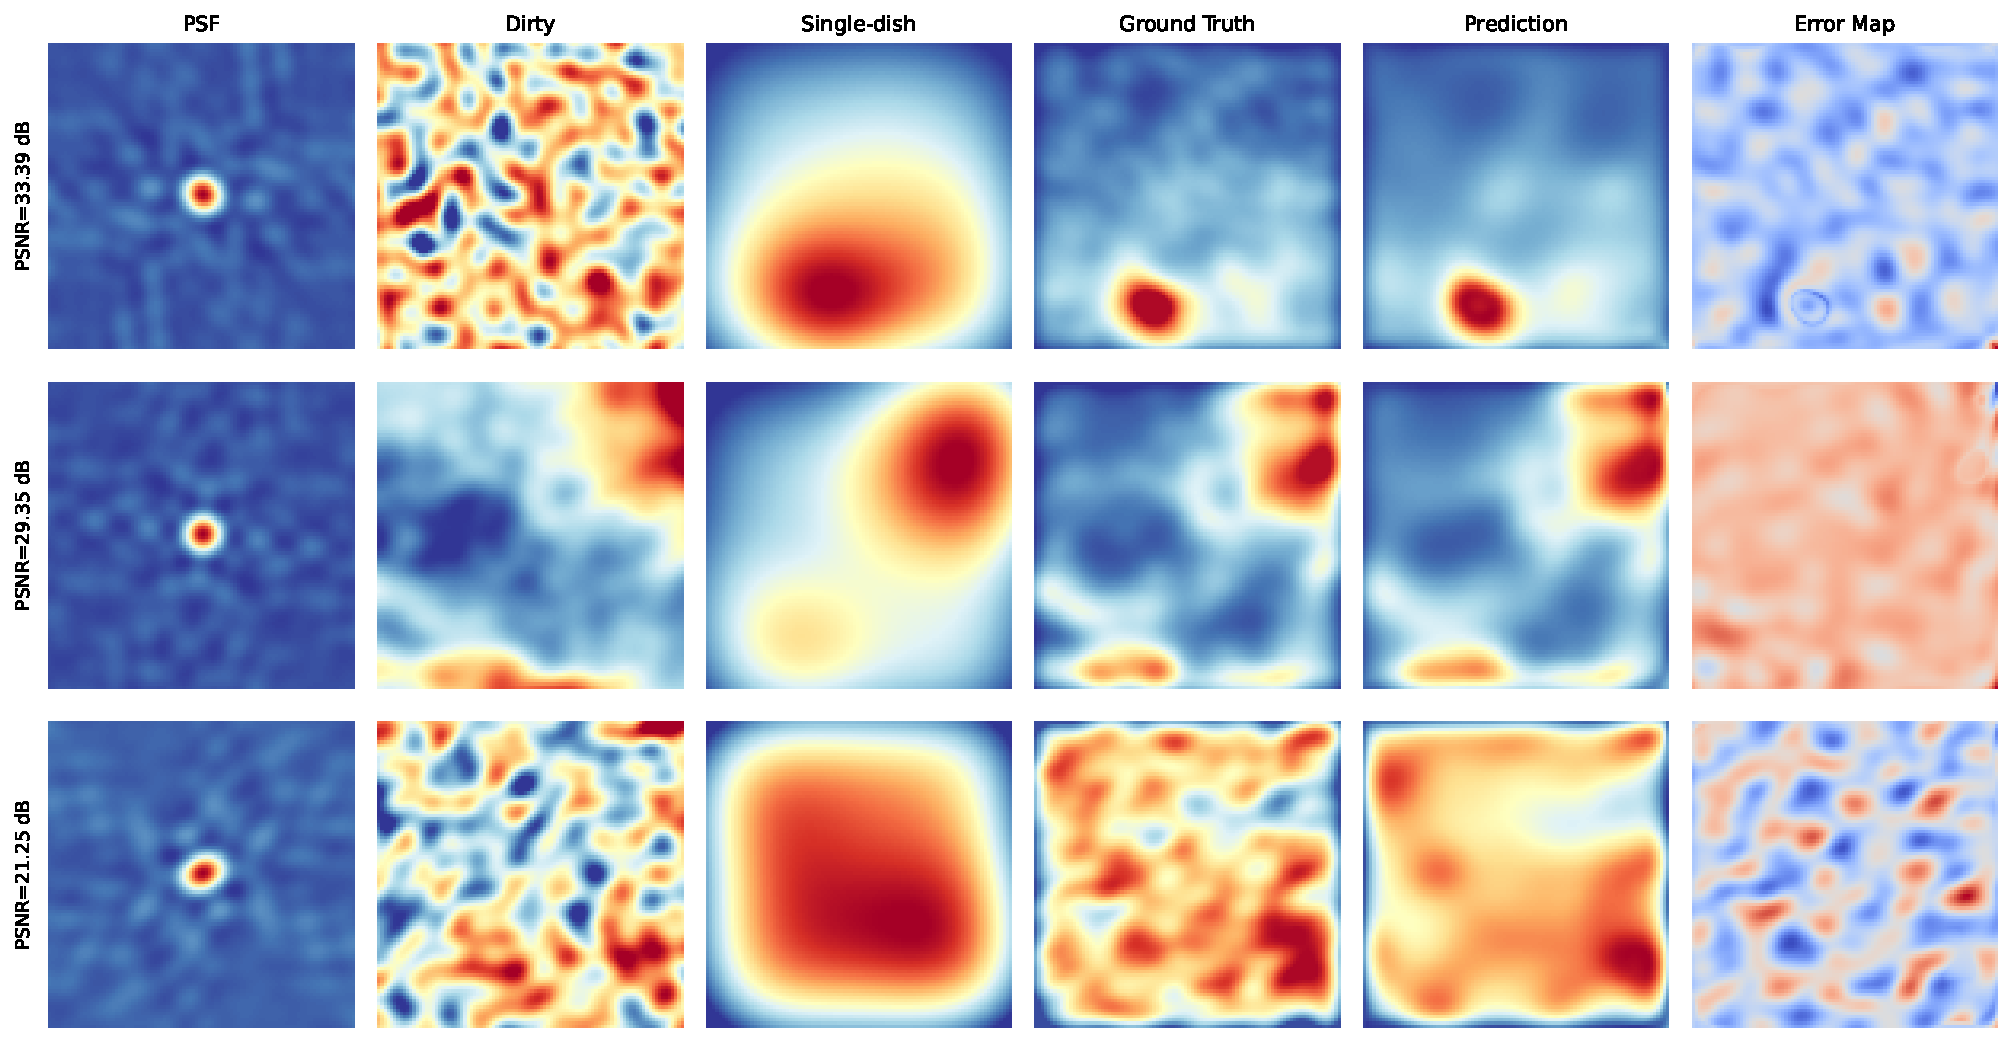
\includegraphics[width=\textwidth]{figures/qualitative_results.pdf}
	\caption{Qualitative reconstruction examples.
		Each row shows (left to right): PSF, dirty image, single-dish image, reference target, model prediction, and error map.
		Top: high-PSNR example ($>$30\,dB). Middle: medium-PSNR example ($\sim$26\,dB). Bottom: low-PSNR example ($<$20\,dB).}
	\label{fig:qualitative}
\end{figure*}

% ============================================================
\clearpage
\section{Discussion}
\label{sec:discussion}

\subsection{The Critical Role of Normalization}

The experiments show that normalization is not a secondary implementation detail but a first-order modeling decision for radio reconstruction.
Independent per-sample, per-modality normalization preserves the usable contrast of the reference target and stabilizes optimization across samples with widely varying flux scales.
The contrast with joint or ratio-preserving schemes suggests a broader lesson for scientific imaging: when the target occupies only a small fraction of the raw amplitude range, physically intuitive but overly coupled normalization can remove the contrast required by supervised learning.

\subsection{Structure-Aware Losses vs.\ Architecture Complexity}

A data-driven comparison shows that structure-aware loss terms (+1.24\,dB from gradient and Laplacian losses alone) provide a larger isolated gain than a fourfold increase in model parameters (+0.46\,dB).
For this benchmark, injecting morphology-aware structure through the objective is therefore more effective than relying on generic capacity scaling alone.
The best result is obtained when both are combined, suggesting that larger models become most useful after the optimization target is aligned with the spatial statistics of radio images.

\subsection{CNN vs.\ Transformer Architectures}

U-Net models outperform the evaluated Transformer variants at comparable experimental maturity.
This behavior is plausible for at least three reasons: the images are relatively small ($192 \times 192$), the task is dominated by local and multi-scale structure recovery, and skip-connected encoder--decoder pathways are well matched to deconvolution-like problems.
The SwinIR results nevertheless become competitive once capacity and training protocol are improved, so the present evidence should be interpreted as favoring convolutional inductive bias for this dataset rather than as a general negative result for Transformers in radio imaging.

\subsection{Effectiveness of Single-Dish (SD) Data}

Including SD data as an explicit conditioning channel is important for this task, particularly for large-scale and low-spatial-frequency structure recovery.
Because interferometers miss short spacings, multiple sky models can remain compatible with the same dirty image once compact structure has been fitted.
In the proposed multimodal formulation, the SD channel reduces that ambiguity by providing total-power information, while the PSF and dirty channels preserve the instrumental response and high-frequency constraints.

The architecture-matched ablation indicates that the SD channel is not merely correlated with stronger model configurations; it is a major source of performance gain under the current benchmark.
That conclusion is especially relevant for applications involving diffuse or extended structures, where large-scale morphology can strongly affect reconstruction utility.
Future work should quantify this effect more directly using low-frequency residual spectra and robustness tests against SD calibration or noise perturbations.

\subsection{Comparison with Classical Deconvolution}

The CASA \texttt{tclean} baselines provide a classical-imaging reference point for the simulated benchmark.
Both H{\"o}gbom and multi-scale \texttt{tclean} improve on the dirty-image input but remain far below the supervised multimodal models under the reported normalized metrics.
This gap should be interpreted in context: the learned models are trained directly against the benchmark reference target and have access to SD information, whereas the \texttt{tclean} references use the interferometric measurement set and do not use the auxiliary SD channel.
The comparison therefore supports the narrower methodological claim that SD-conditioned learned reconstruction can recover the benchmark target more accurately under this protocol, rather than implying that a single \texttt{tclean} parameter setting is globally optimal for radio imaging.

\subsection{Limitations and Future Work}

Several limitations remain.
First, the benchmark is based on simulated observations from a single telescope configuration (VLA D at 1.42\,GHz), so cross-array and cross-configuration generalization still need to be demonstrated.
Second, the supervised target is a benchmark imaging product rather than a directly observed true sky image, so the reported metrics measure agreement with that reference product.
Third, the current $192 \times 192$ image size is smaller than many practical radio-imaging products, and scaling to larger fields will require more careful treatment of memory, tiling, and long-range consistency.
Fourth, the method conditions on the PSF but does not yet enforce the forward measurement equation during training in a fully differentiable end-to-end manner.
Fifth, the broad PSNR spread indicates that low-reference-range samples remain a difficult regime and may require adaptive weighting or curriculum strategies.
Finally, a harmonized comparison with visibility-conditioned diffusion or unrolled inverse-problem methods is still missing and should be considered a priority for future benchmarking.

% ============================================================
\section{Conclusion}
\label{sec:conclusion}

This work studied radio interferometric reconstruction as a domain-specific multimodal computational imaging problem and evaluated a structure-aware supervised learning framework under a unified benchmark.
The results support several conclusions at the intersection of learning-based image restoration and radio-interferometric imaging:

\begin{enumerate}
	\item Per-sample, per-modality normalization is critical for stable learning when radio inputs and benchmark targets span very different dynamic ranges.
	\item Combining pixel, frequency, gradient, and Laplacian losses improves reconstruction quality more effectively than increasing model capacity alone, showing the value of structure-aware objectives for sparse Fourier imaging.
	\item The best-performing model, a larger U-Net with the composite objective, reaches 28.46\,dB PSNR and 0.836 SSIM on the shared 1,272-sample evaluation split.
	\item CASA \texttt{tclean} provides a useful classical deconvolution reference point, while the learned one-pass models achieve substantially higher agreement with the benchmark target under the reported protocol.
	\item Architecture-matched ablations show that the auxiliary SD channel provides strong complementary short-spacing information, with a 12.9--14.0\,dB PSNR penalty when it is removed.
	\item Remaining failure cases concentrate in low-reference-range targets, suggesting that adaptive weighting, curriculum learning, or uncertainty-aware training may further improve robustness.
\end{enumerate}

Overall, the study suggests that high-fidelity learned reconstruction depends not only on architecture choice, but also on how domain structure is represented through normalization, PSF/SD conditioning, loss design, and benchmark discipline.
The proposed framework provides a practical one-pass reconstruction model after training and a reusable experimental template for multimodal image restoration problems with sparse measurements and physically meaningful auxiliary observations.

\section{Code Availability}

Code, configuration files, evaluation scripts, figure-data summaries, and reproducibility notes for the main comparisons are available at \url{https://github.com/arctanbell/radio_recon.git}.

% ============================================================
\appendix

\section{Reproducibility Notes}
\label{sec:appendix_repro}

To improve reproducibility, the principal comparisons are tied to a deterministic seed-42 split protocol, explicit normalization rules, configuration-recorded loss weights, and checkpoint-based evaluation.
Loss weights are configuration-specific rather than universal defaults; the paper reports the relevant settings in the method description and uses the archived configuration files as the source of record.
Unless explicitly stated otherwise, results are reported on the shared 1,272-sample evaluation split so that architecture, loss, and modality comparisons remain directly comparable.

\section{Comparative Positioning with Existing Methods}
\label{sec:appendix_comparison}

To make the relationship with prior methods explicit, Table~\ref{tab:appendix_method_comparison} summarizes key differences in input modality, learned prior, measurement-model use, and inference profile.
This table is intended as a protocol-level comparison rather than a claim of direct numerical superiority.
Strict numerical benchmarking requires harmonized datasets, preprocessing, normalization, and evaluation metrics, which is left as future work.

\begin{table*}[t]
	\centering
	\footnotesize
	\setlength{\tabcolsep}{3pt}
	\renewcommand{\arraystretch}{1.12}
	\caption{Protocol-level comparison across selected radio-interferometric reconstruction approaches.
		``Runtime profile'' indicates practical inference style rather than a fixed benchmark value.
	}
	\label{tab:appendix_method_comparison}
	\resizebox{\textwidth}{!}{%
	\begin{tabular}{llllll}
		\toprule
			Method                                           & Input                                      & Learned / engineered prior                         & Measurement-model use                         & Inference profile                   & Note \\
		\midrule
		CLEAN / MS-CLEAN \citep{Hogbom1974,Cornwell2008} & Visibilities or dirty image + PSF          & Handcrafted sparse model            & Iterative measurement-model deconvolution       & Iterative; tuning-sensitive        & Standard classical baseline \\
		WSClean pipeline \citep{Offringa2014}            & Visibilities                              & Engineered imaging heuristics       & Practical wide-field imaging pipeline           & Efficient, still iterative         & Survey-oriented implementation \\
		CNN image-domain learning \citep{Connor2022,Schmidt2022,Geyer2023,Zhou2025UNet} & Dirty / Fourier data & Supervised image prior & Usually indirect or task-dependent             & One-pass after training   & Closest dirty-to-target family \\
		AIRI / PnP \citep{Terris2022,Terris2025AIRI}     & Visibilities                              & Learned denoising regularizer       & Embedded in optimization with data fidelity      & Iterative learned regularization   & Measurement-consistent learned prior \\
		VIC-DDPM \citep{Wang2023VICDDPM}                 & Visibility + dirty image                  & Conditional diffusion prior         & Measurement-related conditioning                 & Sampling-based generation          & Strong faint-source/detail recovery \\
		R2D2 series \citep{Aghabiglou2024}               & Residual measurement information          & DNN residual series                 & Physics-aware learned reconstruction            & Learned iterative behavior         & Precision radio imaging focus \\
		This work                                        & PSF + dirty + SD image                    & Supervised multimodal prior    & PSF-conditioned image-domain objective & One-pass inference       & Explicit SD conditioning \\
		\bottomrule
	\end{tabular}}
\end{table*}

\subsection{Recommended Fair-Benchmark Protocol}

For future reproducible comparison against diffusion, unrolled, and classical methods, the following protocol is recommended:
\begin{itemize}
	\item identical archived train/validation/evaluation sample lists and identical normalization rules;
	\item reporting both full-test and reference-target-range-stratified metrics;
	\item adding runtime and memory in addition to PSNR/SSIM;
	\item explicitly documenting whether visibilities are used at inference time;
	\item for multimodal methods, adding explicit \texttt{w/o SD} and SD-noise robustness ablations;
	\item for SD-focused analysis, reporting low-frequency reconstruction metrics (e.g., radial FFT-band error at small $|\mathbf{u}|$) and large-scale-structure residual maps.
\end{itemize}

\begin{acknowledgments}
	This work was supported by Shanghai University and Tsinghua University.
	Computations were performed on a workstation equipped with 8$\times$ NVIDIA RTX 4090 GPUs.
	The use of CASA for generating the simulated radio observations is acknowledged.
\end{acknowledgments}

\vspace{5mm}
\facilities{VLA (simulated)}
\software{PyTorch \citep{Paszke2019}, CASA \citep{CASA2022}, astropy \citep{Astropy2022}, scikit-image}

\bibliographystyle{aasjournal}
\bibliography{references}

\end{document}
